\begin{frame}
\frametitle{Project Goals}

The goal of the WCRL Communication Theory Cloud (WCTC) is to provide researchers in communication theory
access to high-performance computing resources for simulation of communication systems.

\vspace{5mm}

\textbf{Features}
\begin{itemize_loose}
\item Implement simulation logic using the WCRL Coded Modulation Library (CML).
\item Utilize a 384-core computing cluster for computational power.
\item Accessible to researchers through a web interface.
\end{itemize_loose}
\end{frame}


% cml
\begin{frame}
\frametitle{Coded Modulation Library}

\textbf{Introduction}
\begin{itemize}
\item Library of communication system simulations developed at WVU.
\item Implemented using MATLAB and C-mex.
\item Free software (licensed under lesser GPL)
\item Download from \url{http://code.google.com/p/iscml/wiki/Cml}
\end{itemize}

\vspace{5mm}
\textbf{Brief list of features}
\begin{itemize}
\item Modulation: PSK, QAM, APSK, CPM (CPFSK)
\item Channel Coding: convolutional, turbo, BTC, LDPC, Hybrid-ARQ
\item Information theoretic bounds (channel capacity; outage probability)
\item TWRC physical-layer network coding: noncoherent FSK relay receiver
\end{itemize}
\end{frame}



%cluster
\begin{frame}
\frametitle{WCRL Computing Cluster}

\begin{columns}[c]

\column{0.6\textwidth}
\begin{itemize}
\item Located on WVU Engineering Campus.
\item 21 rack-mounted servers.
\item Processing cores per server: 8, 16 or 32.
\item Total processing cores: \textbf{384}.
\item Hosts WCTC web interface and simulation logic.
\item Performance stats available at
\\ \url{http://wcrlcluster.csee.wvu.edu/ganglia}
\end{itemize}

\column{0.4\textwidth}
  \begin{figure}
    \centering
    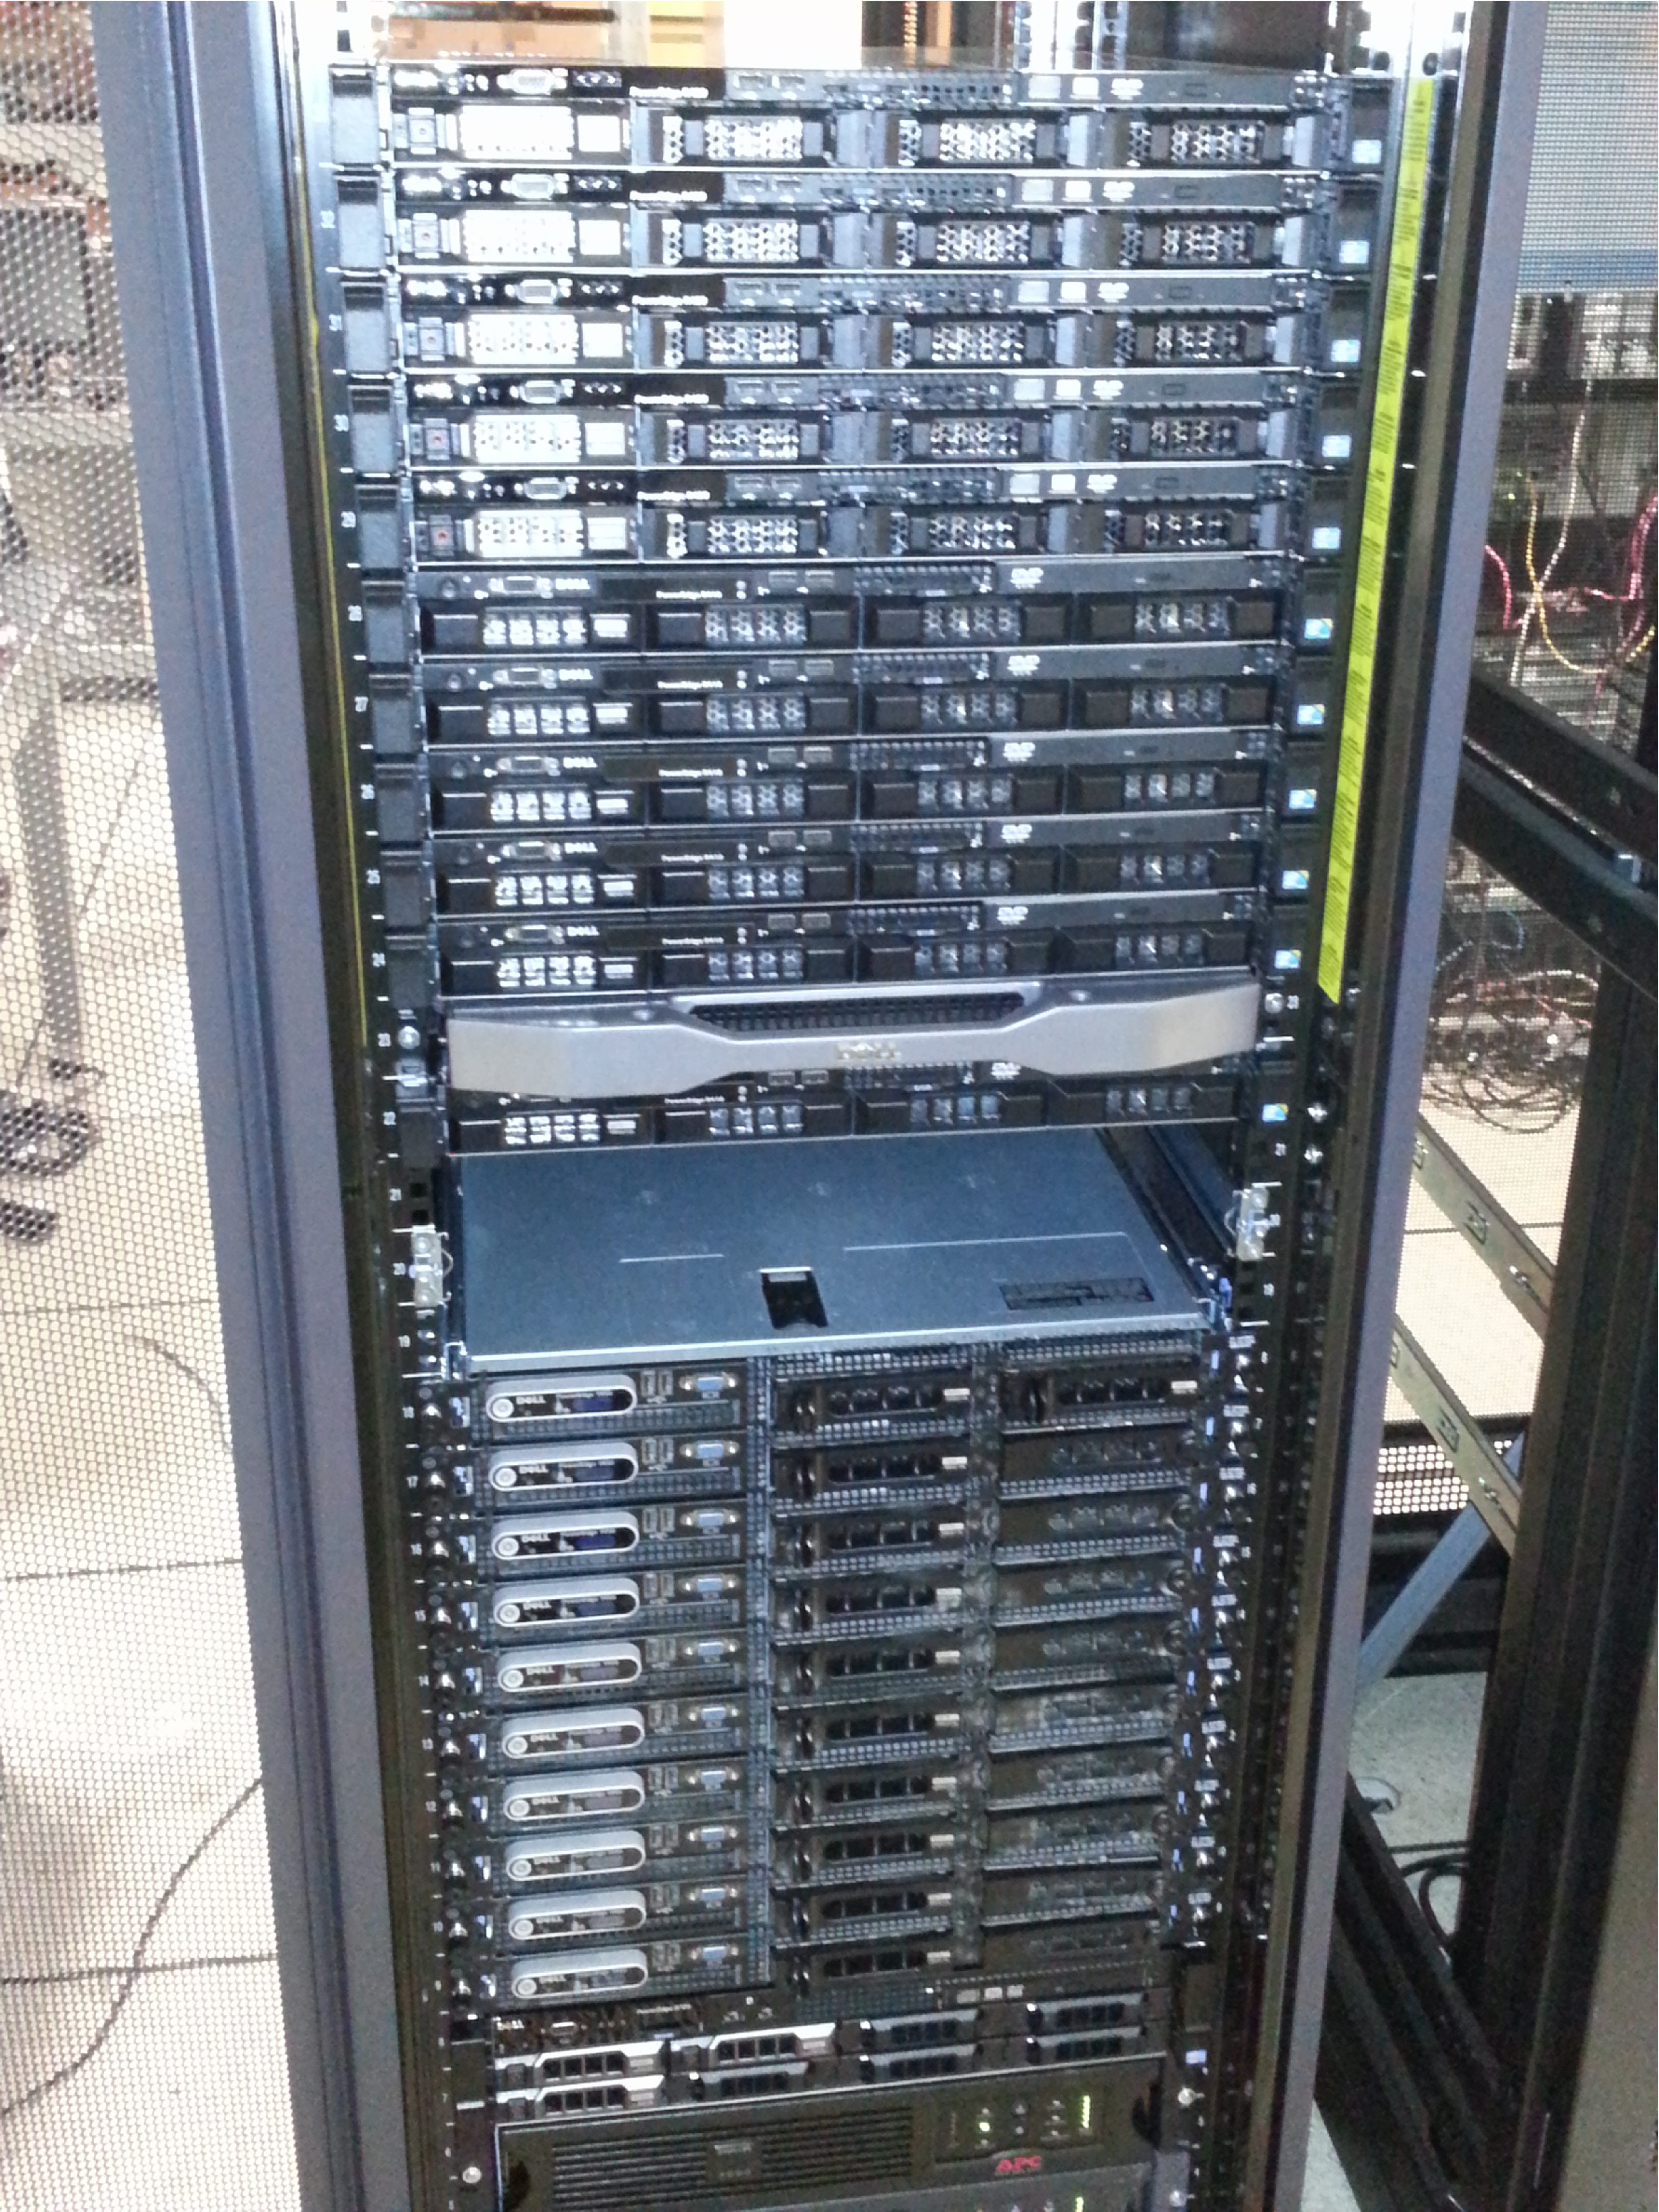
\includegraphics[width=.8\textwidth]{cluster}
  \end{figure}


\end{columns}

\end{frame}
